% % 


Pattern recognition is an applied science that draws from a variety of mathematical fields.
Principal component analysis (PCA) is an unsupervised learning technique that can be used to reveal patterns in high-dimensional data.
The transformation used in the PCA algorithm resembles the singular value decomposition (SVD) in linear algebra and the Karhunen-Loève transform (KLT) in stochastic processes.
Borrowing results from these different approaches, we can start to generalize the PCA algorithm.
The kernel trick from machine learning can be used to create a nonlinear algorithm from a linear one.
In particular, the kernel trick can be applied to PCA.
Kernel PCA is a nonlinear version of PCA that maps data to a suitable Hilbert space and attempts to find patterns in this new context.

We will begin this paper by deriving the PCA transform in \Cref{sec:principal-component-analysis}.
Part of this work depends on results from the SVD and is discussed in \Cref{sub:singular-value-decomposition}.
The PCA section is concluded with examples.
In \Cref{sec:reproducing-kernel-hilbert-space}, we justify the kernel trick.
This prompts the discussion of reproducing kernel Hilbert spaces, Mercer's theorem, the Moore-Aronszajn theorem, and the Riesz representation theorem.
Last, the kernel PCA algorithm is derived in \Cref{sec:kernel-pca}.

% % TODO: Decide on regression intro
In linear regression, the equation of a line \(y = a_0 + a_1 x\) is used to model observations based on training data.
Here, the input variable \(x\) is used to predict the response variable \(y\).
The parameters \(a_0\) and \(a_1\) are chosen such that the residual error\footnote{The residual for a given observation \(\left(x^{(i)},y^{(i)}\right)\) is \(\left|y^{(i)} - \left(a_0 + a_1 x^{(i)}\right)\right|\).} is minimized.
It seems natural to model data using polyomial equations in a similar way, that is, determine \(a_0, a_1, \dots, a_n\) such that
\begin{equation}
    \label{eqn:polynomial-regression}
    y = a_0 + a_1 x + a_2 x^2 + \dots + a_n x^n
\end{equation}
minimizes the residual error.

In multiple linear regression, the equation of a hyperplane
\begin{equation}
    \label{eqn:multiple-linear-regression}
    y = a_0 + a_1 x_1 + a_2 x_2 + \dots + a_n x_n
\end{equation}
is used to predict \(y\) using inputs \(x_1, x_2, \dots x_n\).
It follows that these observations are points in \(n + 1\) dimensions.

% \begin{example}
%     \label{eg:regression}
%     Suppose we have a set of points \(\left\{\left(x^{(i)}, y^{(i)}\right)\right\}_{i=1}^{k}\) in \(\RR^2\).
\begin{figure}
    \centering
    % This file was created by matlab2tikz.
%
%The latest updates can be retrieved from
%  http://www.mathworks.com/matlabcentral/fileexchange/22022-matlab2tikz-matlab2tikz
%where you can also make suggestions and rate matlab2tikz.
%
\definecolor{mycolor1}{rgb}{0.00000,0.44700,0.74100}%
\definecolor{mycolor2}{rgb}{0.85000,0.32500,0.09800}%
%
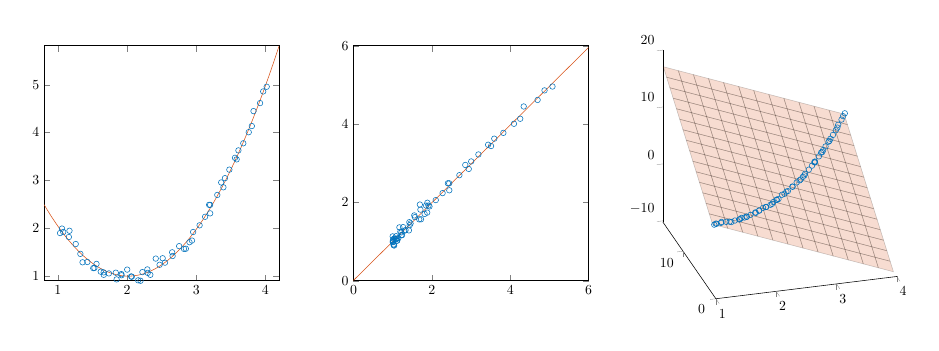
\begin{tikzpicture}[scale=.5]

\begin{axis}[%
width=2.351in,
height=2.351in,
at={(1.432in,0.692in)},
scale only axis,
xmin=0.8,
xmax=4.2,
ymin=0.899321373319454,
ymax=5.81637386238712,
axis background/.style={fill=white}
]
\addplot [color=mycolor1, only marks, mark=o, mark options={solid, mycolor1}, forget plot]
  table[row sep=crcr]{%
1.03102364618709	1.89635200608252\\
1.05874710866312	1.99081508150367\\
1.07666904385065	1.91861076322039\\
1.16700088292618	1.94476477636428\\
1.15852136521559	1.81443225670274\\
1.2573342402677	1.6672445960115\\
1.32425316409503	1.46193166896814\\
1.35639125095251	1.28539362155645\\
1.426390314927	1.29190594605978\\
1.51116628754242	1.16317920678518\\
1.52771797346067	1.16665342088936\\
1.55800752339787	1.25087120537306\\
1.61924984519265	1.08929287399078\\
1.66276456066876	1.02421642799269\\
1.66055829489539	1.07428789900092\\
1.73750766340902	1.05281355009515\\
1.83674063474356	1.06758706338948\\
1.84869247383361	0.927630367762595\\
1.91747269832344	1.03854250275448\\
1.91980499776142	1.01423324648185\\
2.00193550226933	1.13244229108506\\
2.06800875847557	0.98330814258723\\
2.05915455135406	0.990051396490358\\
2.1604277789588	0.908601490469625\\
2.19454470344622	0.899321373319454\\
2.22181395702176	1.0802522633897\\
2.29887400433542	1.0643767640201\\
2.29311086519133	1.13628838486694\\
2.33616069695452	1.02373787382925\\
2.41469230007855	1.36282093678026\\
2.47028403338547	1.2333901421078\\
2.51480903018198	1.3697316642467\\
2.54823716631414	1.27787197059576\\
2.65864684268995	1.41756546923059\\
2.652174488392	1.49433675309514\\
2.7533065654767	1.62304645873151\\
2.82361200029074	1.56631122687407\\
2.84993319641058	1.56911713696776\\
2.90279326280176	1.70524889840619\\
2.93865528830231	1.73949641810109\\
2.95551971666823	1.91897498779834\\
3.04868544243925	2.05861606463079\\
3.12882475635046	2.23744425724559\\
3.2021473479784	2.30906193331213\\
3.18709381272722	2.48714846308874\\
3.20118031790591	2.48677526727991\\
3.3049904247738	2.69403776037719\\
3.36128797731352	2.95522296897976\\
3.39319148605881	2.85358457032387\\
3.41553263131144	3.04520265961224\\
3.56072997798632	3.4707221841804\\
3.47921429467124	3.22300037122612\\
3.584700838626	3.438352021179\\
3.6103512322757	3.62591511616815\\
3.6809161525102	3.77399094847704\\
3.75953554257179	4.00632071052316\\
3.80414143923349	4.13459951411797\\
3.82867794775566	4.44784460055639\\
3.92331010580159	4.61452734184493\\
3.96867181772516	4.85837734147937\\
4.01942142653548	4.95719769247658\\
};
\addplot [color=mycolor2, forget plot]
  table[row sep=crcr]{%
0.8	2.49166207857362\\
0.85	2.37121960692234\\
0.9	2.25583192010692\\
0.95	2.14549901812737\\
1	2.04022090098368\\
1.05	1.93999756867586\\
1.1	1.84482902120391\\
1.15	1.75471525856781\\
1.2	1.66965628076759\\
1.25	1.58965208780323\\
1.3	1.51470267967473\\
1.35	1.4448080563821\\
1.4	1.37996821792533\\
1.45	1.32018316430443\\
1.5	1.26545289551939\\
1.55	1.21577741157022\\
1.6	1.17115671245692\\
1.65	1.13159079817948\\
1.7	1.0970796687379\\
1.75	1.06762332413219\\
1.8	1.04322176436235\\
1.85	1.02387498942837\\
1.9	1.00958299933025\\
1.95	1.000345794068\\
2	0.996163373641616\\
2.05	0.997035738051095\\
2.1	1.00296288729644\\
2.15	1.01394482137765\\
2.2	1.02998154029473\\
2.25	1.05107304404767\\
2.3	1.07721933263647\\
2.35	1.10842040606114\\
2.4	1.14467626432168\\
2.45	1.18598690741808\\
2.5	1.23235233535035\\
2.55	1.28377254811848\\
2.6	1.34024754572247\\
2.65	1.40177732816233\\
2.7	1.46836189543806\\
2.75	1.54000124754965\\
2.8	1.61669538449711\\
2.85	1.69844430628043\\
2.9	1.78524801289962\\
2.95	1.87710650435467\\
3	1.97401978064558\\
3.05	2.07598784177237\\
3.1	2.18301068773501\\
3.15	2.29508831853353\\
3.2	2.4122207341679\\
3.25	2.53440793463815\\
3.3	2.66164991994425\\
3.35	2.79394669008623\\
3.4	2.93129824506406\\
3.45	3.07370458487777\\
3.5	3.22116570952733\\
3.55	3.37368161901277\\
3.6	3.53125231333406\\
3.65	3.69387779249123\\
3.7	3.86155805648426\\
3.75	4.03429310531315\\
3.8	4.21208293897791\\
3.85	4.39492755747853\\
3.9	4.58282696081502\\
3.95	4.77578114898737\\
4	4.97379012199559\\
4.05	5.17685387983967\\
4.1	5.38497242251963\\
4.15	5.59814575003544\\
4.2	5.81637386238712\\
};
\end{axis}

\begin{axis}[%
width=2.351in,
height=2.351in,
at={(4.526in,0.692in)},
scale only axis,
xmin=0,
xmax=6,
ymin=0,
ymax=6,
axis background/.style={fill=white}
]
\addplot [color=mycolor1, only marks, mark=o, mark options={solid, mycolor1}, forget plot]
  table[row sep=crcr]{%
1.93891517424856	1.89635200608252\\
1.88595700545003	1.99081508150367\\
1.85254005458367	1.91861076322039\\
1.69388752904577	1.94476477636428\\
1.70808629279864	1.81443225670274\\
1.55155243067876	1.6672445960115\\
1.45663378623558	1.46193166896814\\
1.41423222185048	1.28539362155645\\
1.32902807080954	1.29190594605978\\
1.23895839843506	1.16317920678518\\
1.2230503125921	1.16665342088936\\
1.19535734937288	1.25087120537306\\
1.14497068038582	1.08929287399078\\
1.11372774154094	1.02421642799269\\
1.11522067116432	1.07428789900092\\
1.06890222676899	1.05281355009515\\
1.02665362034394	1.06758706338948\\
1.02289396747459	0.927630367762595\\
1.00681075552201	1.03854250275448\\
1.00643123838405	1.01423324648185\\
1.00000374616903	1.13244229108506\\
1.00462519122939	0.98330814258723\\
1.0034992609459	0.990051396490358\\
1.02573707226165	0.908601490469625\\
1.03784764163898	0.899321373319454\\
1.04920143152965	1.0802522633897\\
1.08932567046749	1.0643767640201\\
1.08591397929321	1.13628838486694\\
1.11300401417695	1.02373787382925\\
1.17196970374444	1.36282093678026\\
1.22116707205731	1.2333901421078\\
1.26502833755691	1.3697316642467\\
1.30056399052816	1.27787197059576\\
1.43381566338544	1.41756546923059\\
1.42533156330936	1.49433675309514\\
1.5674707815903	1.62304645873151\\
1.67833672702291	1.56631122687407\\
1.72238643836071	1.56911713696776\\
1.81503567536025	1.70524889840619\\
1.88107375025789	1.73949641810109\\
1.91301792894173	1.91897498779834\\
2.09974115718401	2.05861606463079\\
2.27424533054968	2.23744425724559\\
2.4451582462515	2.30906193331213\\
2.40919172021524	2.48714846308874\\
2.44283415612453	2.48677526727991\\
2.70300000875131	2.69403776037719\\
2.85310495717834	2.95522296897976\\
2.94098251682676	2.85358457032387\\
3.00373263030748	3.04520265961224\\
3.43587806418517	3.4707221841804\\
3.18807492955975	3.22300037122612\\
3.51127674794195	3.438352021179\\
3.59323109129186	3.62591511616815\\
3.82547911176969	3.77399094847704\\
4.09596532557341	4.00632071052316\\
4.25492633275947	4.13459951411797\\
4.34406303660786	4.44784460055639\\
4.69912176307854	4.61452734184493\\
4.87566872590529	4.85837734147937\\
5.0780628979506	4.95719769247658\\
};
\addplot [color=mycolor2, forget plot]
  table[row sep=crcr]{%
0	0.00977935819441985\\
0.05	0.0593099862633467\\
0.1	0.108840614332273\\
0.15	0.1583712424012\\
0.2	0.207901870470127\\
0.25	0.257432498539054\\
0.3	0.306963126607981\\
0.35	0.356493754676908\\
0.4	0.406024382745834\\
0.45	0.455555010814761\\
0.5	0.505085638883688\\
0.55	0.554616266952615\\
0.6	0.604146895021542\\
0.65	0.653677523090468\\
0.7	0.703208151159395\\
0.75	0.752738779228322\\
0.8	0.802269407297249\\
0.85	0.851800035366176\\
0.9	0.901330663435102\\
0.95	0.950861291504029\\
1	1.00039191957296\\
1.05	1.04992254764188\\
1.1	1.09945317571081\\
1.15	1.14898380377974\\
1.2	1.19851443184866\\
1.25	1.24804505991759\\
1.3	1.29757568798652\\
1.35	1.34710631605544\\
1.4	1.39663694412437\\
1.45	1.4461675721933\\
1.5	1.49569820026222\\
1.55	1.54522882833115\\
1.6	1.59475945640008\\
1.65	1.644290084469\\
1.7	1.69382071253793\\
1.75	1.74335134060686\\
1.8	1.79288196867579\\
1.85	1.84241259674471\\
1.9	1.89194322481364\\
1.95	1.94147385288257\\
2	1.99100448095149\\
2.05	2.04053510902042\\
2.1	2.09006573708935\\
2.15	2.13959636515827\\
2.2	2.1891269932272\\
2.25	2.23865762129613\\
2.3	2.28818824936505\\
2.35	2.33771887743398\\
2.4	2.38724950550291\\
2.45	2.43678013357183\\
2.5	2.48631076164076\\
2.55	2.53584138970969\\
2.6	2.58537201777861\\
2.65	2.63490264584754\\
2.7	2.68443327391647\\
2.75	2.73396390198539\\
2.8	2.78349453005432\\
2.85	2.83302515812325\\
2.9	2.88255578619217\\
2.95	2.9320864142611\\
3	2.98161704233003\\
3.05	3.03114767039895\\
3.1	3.08067829846788\\
3.15	3.13020892653681\\
3.2	3.17973955460574\\
3.25	3.22927018267466\\
3.3	3.27880081074359\\
3.35	3.32833143881252\\
3.4	3.37786206688144\\
3.45	3.42739269495037\\
3.5	3.4769233230193\\
3.55	3.52645395108822\\
3.6	3.57598457915715\\
3.65	3.62551520722608\\
3.7	3.675045835295\\
3.75	3.72457646336393\\
3.8	3.77410709143286\\
3.85	3.82363771950178\\
3.9	3.87316834757071\\
3.95	3.92269897563964\\
4	3.97222960370856\\
4.05	4.02176023177749\\
4.1	4.07129085984642\\
4.15	4.12082148791534\\
4.2	4.17035211598427\\
4.25	4.2198827440532\\
4.3	4.26941337212213\\
4.35	4.31894400019105\\
4.4	4.36847462825998\\
4.45	4.41800525632891\\
4.5	4.46753588439783\\
4.55	4.51706651246676\\
4.6	4.56659714053569\\
4.65	4.61612776860461\\
4.7	4.66565839667354\\
4.75	4.71518902474247\\
4.8	4.76471965281139\\
4.85	4.81425028088032\\
4.9	4.86378090894925\\
4.95	4.91331153701817\\
5	4.9628421650871\\
5.05	5.01237279315603\\
5.1	5.06190342122495\\
5.15	5.11143404929388\\
5.2	5.16096467736281\\
5.25	5.21049530543173\\
5.3	5.26002593350066\\
5.35	5.30955656156959\\
5.4	5.35908718963852\\
5.45	5.40861781770744\\
5.5	5.45814844577637\\
5.55	5.5076790738453\\
5.6	5.55720970191422\\
5.65	5.60674032998315\\
5.7	5.65627095805208\\
5.75	5.705801586121\\
5.8	5.75533221418993\\
5.85	5.80486284225886\\
5.9	5.85439347032778\\
5.95	5.90392409839671\\
6	5.95345472646564\\
};
\end{axis}

\begin{axis}[%
width=2.351in,
height=2.711in,
at={(7.619in,0.512in)},
scale only axis,
plot box ratio=1 1 1,
xmin=1,
xmax=4.01942142653548,
tick align=outside,
ymin=0,
ymax=16.1557486040925,
zmin=-10.1905643855997,
zmax=20,
view={-16.2617026369184}{24.9729119273008},
axis background/.style={fill=white},
axis x line*=bottom,
axis y line*=left,
axis z line*=left
]
\addplot3 [color=mycolor1, only marks, mark=o, mark options={solid, mycolor1}]
 table[row sep=crcr] {%
1.03102364618709	1.06300975899692	1.89635200608252\\
1.05874710866312	1.12094544010253	1.99081508150367\\
1.07666904385065	1.15921622998628	1.91861076322039\\
1.16700088292618	1.36189106075048	1.94476477636428\\
1.15852136521559	1.34217175366099	1.81443225670274\\
1.2573342402677	1.58088939174955	1.6672445960115\\
1.32425316409503	1.7536464426157	1.46193166896814\\
1.35639125095251	1.83979722566052	1.28539362155645\\
1.426390314927	2.03458933051756	1.29190594605978\\
1.51116628754242	2.28362354860474	1.16317920678518\\
1.52771797346067	2.33392220643477	1.16665342088936\\
1.55800752339787	2.42738744296438	1.25087120537306\\
1.61924984519265	2.62197006115643	1.08929287399078\\
1.66276456066876	2.76478598421597	1.02421642799269\\
1.66055829489539	2.7574538507459	1.07428789900092\\
1.73750766340902	3.01893288040506	1.05281355009515\\
1.83674063474356	3.37361615931818	1.06758706338948\\
1.84869247383361	3.41766386280903	0.927630367762595\\
1.91747269832344	3.67670154881577	1.03854250275448\\
1.91980499776142	3.68565122942973	1.01423324648185\\
2.00193550226933	4.00774575524637	1.13244229108506\\
2.06800875847557	4.27666022513168	0.98330814258723\\
2.05915455135406	4.24011746636215	0.990051396490358\\
2.1604277789588	4.66744818809686	0.908601490469625\\
2.19454470344622	4.81602645542386	0.899321373319454\\
2.22181395702176	4.93645725961667	1.0802522633897\\
2.29887400433542	5.28482168780919	1.0643767640201\\
2.29311086519133	5.25835744005851	1.13628838486694\\
2.33616069695452	5.45764680199503	1.02373787382925\\
2.41469230007855	5.83073890405865	1.36282093678026\\
2.47028403338547	6.10230320559921	1.2333901421078\\
2.51480903018198	6.32426445828482	1.3697316642467\\
2.54823716631414	6.49351265578471	1.27787197059576\\
2.65864684268995	7.06840303414524	1.41756546923059\\
2.652174488392	7.03402951687734	1.49433675309514\\
2.7533065654767	7.58069704349711	1.62304645873151\\
2.82361200029074	7.97278472818587	1.56631122687407\\
2.84993319641058	8.12211922400305	1.56911713696776\\
2.90279326280176	8.42620872656731	1.70524889840619\\
2.93865528830231	8.63569490346712	1.73949641810109\\
2.95551971666823	8.73509679561465	1.91897498779834\\
3.04868544243925	9.29448292694101	2.05861606463079\\
3.12882475635046	9.78954435595154	2.23744425724559\\
3.2021473479784	10.2537476381651	2.30906193331213\\
3.18709381272722	10.1575669711241	2.48714846308874\\
3.20118031790591	10.2475554277482	2.48677526727991\\
3.3049904247738	10.9229617078465	2.69403776037719\\
3.36128797731352	11.2982568664324	2.95522296897976\\
3.39319148605881	11.513748461062	2.85358457032387\\
3.41553263131144	11.6658631555532	3.04520265961224\\
3.56072997798632	12.6787979761304	3.4707221841804\\
3.47921429467124	12.1049321082447	3.22300037122612\\
3.584700838626	12.850080102446	3.438352021179\\
3.6103512322757	13.0346360203946	3.62591511616815\\
3.6809161525102	13.5491437218105	3.77399094847704\\
3.75953554257179	14.1341074958606	4.00632071052316\\
3.80414143923349	14.4714920896934	4.13459951411797\\
3.82867794775566	14.6587748276305	4.44784460055639\\
3.92331010580159	15.3923621862849	4.61452734184493\\
3.96867181772516	15.7503559968059	4.85837734147937\\
4.01942142653548	16.1557486040925	4.95719769247658\\
};
 
\addplot3[%
surf,
fill opacity=0.2, draw opacity=0.2, fill=mycolor2, faceted color=black, z buffer=sort, colormap={mymap}{[1pt] rgb(0pt)=(0.2422,0.1504,0.6603); rgb(1pt)=(0.2444,0.1534,0.6728); rgb(2pt)=(0.2464,0.1569,0.6847); rgb(3pt)=(0.2484,0.1607,0.6961); rgb(4pt)=(0.2503,0.1648,0.7071); rgb(5pt)=(0.2522,0.1689,0.7179); rgb(6pt)=(0.254,0.1732,0.7286); rgb(7pt)=(0.2558,0.1773,0.7393); rgb(8pt)=(0.2576,0.1814,0.7501); rgb(9pt)=(0.2594,0.1854,0.761); rgb(11pt)=(0.2628,0.1932,0.7828); rgb(12pt)=(0.2645,0.1972,0.7937); rgb(13pt)=(0.2661,0.2011,0.8043); rgb(14pt)=(0.2676,0.2052,0.8148); rgb(15pt)=(0.2691,0.2094,0.8249); rgb(16pt)=(0.2704,0.2138,0.8346); rgb(17pt)=(0.2717,0.2184,0.8439); rgb(18pt)=(0.2729,0.2231,0.8528); rgb(19pt)=(0.274,0.228,0.8612); rgb(20pt)=(0.2749,0.233,0.8692); rgb(21pt)=(0.2758,0.2382,0.8767); rgb(22pt)=(0.2766,0.2435,0.884); rgb(23pt)=(0.2774,0.2489,0.8908); rgb(24pt)=(0.2781,0.2543,0.8973); rgb(25pt)=(0.2788,0.2598,0.9035); rgb(26pt)=(0.2794,0.2653,0.9094); rgb(27pt)=(0.2798,0.2708,0.915); rgb(28pt)=(0.2802,0.2764,0.9204); rgb(29pt)=(0.2806,0.2819,0.9255); rgb(30pt)=(0.2809,0.2875,0.9305); rgb(31pt)=(0.2811,0.293,0.9352); rgb(32pt)=(0.2813,0.2985,0.9397); rgb(33pt)=(0.2814,0.304,0.9441); rgb(34pt)=(0.2814,0.3095,0.9483); rgb(35pt)=(0.2813,0.315,0.9524); rgb(36pt)=(0.2811,0.3204,0.9563); rgb(37pt)=(0.2809,0.3259,0.96); rgb(38pt)=(0.2807,0.3313,0.9636); rgb(39pt)=(0.2803,0.3367,0.967); rgb(40pt)=(0.2798,0.3421,0.9702); rgb(41pt)=(0.2791,0.3475,0.9733); rgb(42pt)=(0.2784,0.3529,0.9763); rgb(43pt)=(0.2776,0.3583,0.9791); rgb(44pt)=(0.2766,0.3638,0.9817); rgb(45pt)=(0.2754,0.3693,0.984); rgb(46pt)=(0.2741,0.3748,0.9862); rgb(47pt)=(0.2726,0.3804,0.9881); rgb(48pt)=(0.271,0.386,0.9898); rgb(49pt)=(0.2691,0.3916,0.9912); rgb(50pt)=(0.267,0.3973,0.9924); rgb(51pt)=(0.2647,0.403,0.9935); rgb(52pt)=(0.2621,0.4088,0.9946); rgb(53pt)=(0.2591,0.4145,0.9955); rgb(54pt)=(0.2556,0.4203,0.9965); rgb(55pt)=(0.2517,0.4261,0.9974); rgb(56pt)=(0.2473,0.4319,0.9983); rgb(57pt)=(0.2424,0.4378,0.9991); rgb(58pt)=(0.2369,0.4437,0.9996); rgb(59pt)=(0.2311,0.4497,0.9995); rgb(60pt)=(0.225,0.4559,0.9985); rgb(61pt)=(0.2189,0.462,0.9968); rgb(62pt)=(0.2128,0.4682,0.9948); rgb(63pt)=(0.2066,0.4743,0.9926); rgb(64pt)=(0.2006,0.4803,0.9906); rgb(65pt)=(0.195,0.4861,0.9887); rgb(66pt)=(0.1903,0.4919,0.9867); rgb(67pt)=(0.1869,0.4975,0.9844); rgb(68pt)=(0.1847,0.503,0.9819); rgb(69pt)=(0.1831,0.5084,0.9793); rgb(70pt)=(0.1818,0.5138,0.9766); rgb(71pt)=(0.1806,0.5191,0.9738); rgb(72pt)=(0.1795,0.5244,0.9709); rgb(73pt)=(0.1785,0.5296,0.9677); rgb(74pt)=(0.1778,0.5349,0.9641); rgb(75pt)=(0.1773,0.5401,0.9602); rgb(76pt)=(0.1768,0.5452,0.956); rgb(77pt)=(0.1764,0.5504,0.9516); rgb(78pt)=(0.1755,0.5554,0.9473); rgb(79pt)=(0.174,0.5605,0.9432); rgb(80pt)=(0.1716,0.5655,0.9393); rgb(81pt)=(0.1686,0.5705,0.9357); rgb(82pt)=(0.1649,0.5755,0.9323); rgb(83pt)=(0.161,0.5805,0.9289); rgb(84pt)=(0.1573,0.5854,0.9254); rgb(85pt)=(0.154,0.5902,0.9218); rgb(86pt)=(0.1513,0.595,0.9182); rgb(87pt)=(0.1492,0.5997,0.9147); rgb(88pt)=(0.1475,0.6043,0.9113); rgb(89pt)=(0.1461,0.6089,0.908); rgb(90pt)=(0.1446,0.6135,0.905); rgb(91pt)=(0.1429,0.618,0.9022); rgb(92pt)=(0.1408,0.6226,0.8998); rgb(93pt)=(0.1383,0.6272,0.8975); rgb(94pt)=(0.1354,0.6317,0.8953); rgb(95pt)=(0.1321,0.6363,0.8932); rgb(96pt)=(0.1288,0.6408,0.891); rgb(97pt)=(0.1253,0.6453,0.8887); rgb(98pt)=(0.1219,0.6497,0.8862); rgb(99pt)=(0.1185,0.6541,0.8834); rgb(100pt)=(0.1152,0.6584,0.8804); rgb(101pt)=(0.1119,0.6627,0.877); rgb(102pt)=(0.1085,0.6669,0.8734); rgb(103pt)=(0.1048,0.671,0.8695); rgb(104pt)=(0.1009,0.675,0.8653); rgb(105pt)=(0.0964,0.6789,0.8609); rgb(106pt)=(0.0914,0.6828,0.8562); rgb(107pt)=(0.0855,0.6865,0.8513); rgb(108pt)=(0.0789,0.6902,0.8462); rgb(109pt)=(0.0713,0.6938,0.8409); rgb(110pt)=(0.0628,0.6972,0.8355); rgb(111pt)=(0.0535,0.7006,0.8299); rgb(112pt)=(0.0433,0.7039,0.8242); rgb(113pt)=(0.0328,0.7071,0.8183); rgb(114pt)=(0.0234,0.7103,0.8124); rgb(115pt)=(0.0155,0.7133,0.8064); rgb(116pt)=(0.0091,0.7163,0.8003); rgb(117pt)=(0.0046,0.7192,0.7941); rgb(118pt)=(0.0019,0.722,0.7878); rgb(119pt)=(0.0009,0.7248,0.7815); rgb(120pt)=(0.0018,0.7275,0.7752); rgb(121pt)=(0.0046,0.7301,0.7688); rgb(122pt)=(0.0094,0.7327,0.7623); rgb(123pt)=(0.0162,0.7352,0.7558); rgb(124pt)=(0.0253,0.7376,0.7492); rgb(125pt)=(0.0369,0.74,0.7426); rgb(126pt)=(0.0504,0.7423,0.7359); rgb(127pt)=(0.0638,0.7446,0.7292); rgb(128pt)=(0.077,0.7468,0.7224); rgb(129pt)=(0.0899,0.7489,0.7156); rgb(130pt)=(0.1023,0.751,0.7088); rgb(131pt)=(0.1141,0.7531,0.7019); rgb(132pt)=(0.1252,0.7552,0.695); rgb(133pt)=(0.1354,0.7572,0.6881); rgb(134pt)=(0.1448,0.7593,0.6812); rgb(135pt)=(0.1532,0.7614,0.6741); rgb(136pt)=(0.1609,0.7635,0.6671); rgb(137pt)=(0.1678,0.7656,0.6599); rgb(138pt)=(0.1741,0.7678,0.6527); rgb(139pt)=(0.1799,0.7699,0.6454); rgb(140pt)=(0.1853,0.7721,0.6379); rgb(141pt)=(0.1905,0.7743,0.6303); rgb(142pt)=(0.1954,0.7765,0.6225); rgb(143pt)=(0.2003,0.7787,0.6146); rgb(144pt)=(0.2061,0.7808,0.6065); rgb(145pt)=(0.2118,0.7828,0.5983); rgb(146pt)=(0.2178,0.7849,0.5899); rgb(147pt)=(0.2244,0.7869,0.5813); rgb(148pt)=(0.2318,0.7887,0.5725); rgb(149pt)=(0.2401,0.7905,0.5636); rgb(150pt)=(0.2491,0.7922,0.5546); rgb(151pt)=(0.2589,0.7937,0.5454); rgb(152pt)=(0.2695,0.7951,0.536); rgb(153pt)=(0.2809,0.7964,0.5266); rgb(154pt)=(0.2929,0.7975,0.517); rgb(155pt)=(0.3052,0.7985,0.5074); rgb(156pt)=(0.3176,0.7994,0.4975); rgb(157pt)=(0.3301,0.8002,0.4876); rgb(158pt)=(0.3424,0.8009,0.4774); rgb(159pt)=(0.3548,0.8016,0.4669); rgb(160pt)=(0.3671,0.8021,0.4563); rgb(161pt)=(0.3795,0.8026,0.4454); rgb(162pt)=(0.3921,0.8029,0.4344); rgb(163pt)=(0.405,0.8031,0.4233); rgb(164pt)=(0.4184,0.803,0.4122); rgb(165pt)=(0.4322,0.8028,0.4013); rgb(166pt)=(0.4463,0.8024,0.3904); rgb(167pt)=(0.4608,0.8018,0.3797); rgb(168pt)=(0.4753,0.8011,0.3691); rgb(169pt)=(0.4899,0.8002,0.3586); rgb(170pt)=(0.5044,0.7993,0.348); rgb(171pt)=(0.5187,0.7982,0.3374); rgb(172pt)=(0.5329,0.797,0.3267); rgb(173pt)=(0.547,0.7957,0.3159); rgb(175pt)=(0.5748,0.7929,0.2941); rgb(176pt)=(0.5886,0.7913,0.2833); rgb(177pt)=(0.6024,0.7896,0.2726); rgb(178pt)=(0.6161,0.7878,0.2622); rgb(179pt)=(0.6297,0.7859,0.2521); rgb(180pt)=(0.6433,0.7839,0.2423); rgb(181pt)=(0.6567,0.7818,0.2329); rgb(182pt)=(0.6701,0.7796,0.2239); rgb(183pt)=(0.6833,0.7773,0.2155); rgb(184pt)=(0.6963,0.775,0.2075); rgb(185pt)=(0.7091,0.7727,0.1998); rgb(186pt)=(0.7218,0.7703,0.1924); rgb(187pt)=(0.7344,0.7679,0.1852); rgb(188pt)=(0.7468,0.7654,0.1782); rgb(189pt)=(0.759,0.7629,0.1717); rgb(190pt)=(0.771,0.7604,0.1658); rgb(191pt)=(0.7829,0.7579,0.1608); rgb(192pt)=(0.7945,0.7554,0.157); rgb(193pt)=(0.806,0.7529,0.1546); rgb(194pt)=(0.8172,0.7505,0.1535); rgb(195pt)=(0.8281,0.7481,0.1536); rgb(196pt)=(0.8389,0.7457,0.1546); rgb(197pt)=(0.8495,0.7435,0.1564); rgb(198pt)=(0.86,0.7413,0.1587); rgb(199pt)=(0.8703,0.7392,0.1615); rgb(200pt)=(0.8804,0.7372,0.165); rgb(201pt)=(0.8903,0.7353,0.1695); rgb(202pt)=(0.9,0.7336,0.1749); rgb(203pt)=(0.9093,0.7321,0.1815); rgb(204pt)=(0.9184,0.7308,0.189); rgb(205pt)=(0.9272,0.7298,0.1973); rgb(206pt)=(0.9357,0.729,0.2061); rgb(207pt)=(0.944,0.7285,0.2151); rgb(208pt)=(0.9523,0.7284,0.2237); rgb(209pt)=(0.9606,0.7285,0.2312); rgb(210pt)=(0.9689,0.7292,0.2373); rgb(211pt)=(0.977,0.7304,0.2418); rgb(212pt)=(0.9842,0.733,0.2446); rgb(213pt)=(0.99,0.7365,0.2429); rgb(214pt)=(0.9946,0.7407,0.2394); rgb(215pt)=(0.9966,0.7458,0.2351); rgb(216pt)=(0.9971,0.7513,0.2309); rgb(217pt)=(0.9972,0.7569,0.2267); rgb(218pt)=(0.9971,0.7626,0.2224); rgb(219pt)=(0.9969,0.7683,0.2181); rgb(220pt)=(0.9966,0.774,0.2138); rgb(221pt)=(0.9962,0.7798,0.2095); rgb(222pt)=(0.9957,0.7856,0.2053); rgb(223pt)=(0.9949,0.7915,0.2012); rgb(224pt)=(0.9938,0.7974,0.1974); rgb(225pt)=(0.9923,0.8034,0.1939); rgb(226pt)=(0.9906,0.8095,0.1906); rgb(227pt)=(0.9885,0.8156,0.1875); rgb(228pt)=(0.9861,0.8218,0.1846); rgb(229pt)=(0.9835,0.828,0.1817); rgb(230pt)=(0.9807,0.8342,0.1787); rgb(231pt)=(0.9778,0.8404,0.1757); rgb(232pt)=(0.9748,0.8467,0.1726); rgb(233pt)=(0.972,0.8529,0.1695); rgb(234pt)=(0.9694,0.8591,0.1665); rgb(235pt)=(0.9671,0.8654,0.1636); rgb(236pt)=(0.9651,0.8716,0.1608); rgb(237pt)=(0.9634,0.8778,0.1582); rgb(238pt)=(0.9619,0.884,0.1557); rgb(239pt)=(0.9608,0.8902,0.1532); rgb(240pt)=(0.9601,0.8963,0.1507); rgb(241pt)=(0.9596,0.9023,0.148); rgb(242pt)=(0.9595,0.9084,0.145); rgb(243pt)=(0.9597,0.9143,0.1418); rgb(244pt)=(0.9601,0.9203,0.1382); rgb(245pt)=(0.9608,0.9262,0.1344); rgb(246pt)=(0.9618,0.932,0.1304); rgb(247pt)=(0.9629,0.9379,0.1261); rgb(248pt)=(0.9642,0.9437,0.1216); rgb(249pt)=(0.9657,0.9494,0.1168); rgb(250pt)=(0.9674,0.9552,0.1116); rgb(251pt)=(0.9692,0.9609,0.1061); rgb(252pt)=(0.9711,0.9667,0.1001); rgb(253pt)=(0.973,0.9724,0.0938); rgb(254pt)=(0.9749,0.9782,0.0872); rgb(255pt)=(0.9769,0.9839,0.0805)}, mesh/rows=13]
table[row sep=crcr, point meta=\thisrow{c}] {%
%
x	y	z	c\\
1	1	2.04022090098368	2.04022090098368\\
1	2	3.0511778681567	3.0511778681567\\
1	3	4.06213483532972	4.06213483532972\\
1	4	5.07309180250274	5.07309180250274\\
1	5	6.08404876967576	6.08404876967576\\
1	6	7.09500573684878	7.09500573684878\\
1	7	8.10596270402179	8.10596270402179\\
1	8	9.11691967119481	9.11691967119481\\
1	9	10.1278766383678	10.1278766383678\\
1	10	11.1388336055408	11.1388336055408\\
1	11	12.1497905727139	12.1497905727139\\
1	12	13.1607475398869	13.1607475398869\\
1	13	14.1717045070599	14.1717045070599\\
1	14	15.1826614742329	15.1826614742329\\
1	15	16.1936184414059	16.1936184414059\\
1	16	17.204575408579	17.204575408579\\
1.25	1	1.0209887937684	1.0209887937684\\
1.25	2	2.03194576094142	2.03194576094142\\
1.25	3	3.04290272811444	3.04290272811444\\
1.25	4	4.05385969528746	4.05385969528746\\
1.25	5	5.06481666246048	5.06481666246048\\
1.25	6	6.07577362963349	6.07577362963349\\
1.25	7	7.08673059680651	7.08673059680651\\
1.25	8	8.09768756397953	8.09768756397953\\
1.25	9	9.10864453115255	9.10864453115255\\
1.25	10	10.1196014983256	10.1196014983256\\
1.25	11	11.1305584654986	11.1305584654986\\
1.25	12	12.1415154326716	12.1415154326716\\
1.25	13	13.1524723998446	13.1524723998446\\
1.25	14	14.1634293670176	14.1634293670176\\
1.25	15	15.1743863341907	15.1743863341907\\
1.25	16	16.1853433013637	16.1853433013637\\
1.5	1	0.00175668655312133	0.00175668655312133\\
1.5	2	1.01271365372614	1.01271365372614\\
1.5	3	2.02367062089916	2.02367062089916\\
1.5	4	3.03462758807218	3.03462758807218\\
1.5	5	4.04558455524519	4.04558455524519\\
1.5	6	5.05654152241821	5.05654152241821\\
1.5	7	6.06749848959123	6.06749848959123\\
1.5	8	7.07845545676425	7.07845545676425\\
1.5	9	8.08941242393727	8.08941242393727\\
1.5	10	9.10036939111029	9.10036939111029\\
1.5	11	10.1113263582833	10.1113263582833\\
1.5	12	11.1222833254563	11.1222833254563\\
1.5	13	12.1332402926293	12.1332402926293\\
1.5	14	13.1441972598024	13.1441972598024\\
1.5	15	14.1551542269754	14.1551542269754\\
1.5	16	15.1661111941484	15.1661111941484\\
1.75	1	-1.01747542066216	-1.01747542066216\\
1.75	2	-0.00651845348914115	-0.00651845348914115\\
1.75	3	1.00443851368388	1.00443851368388\\
1.75	4	2.0153954808569	2.0153954808569\\
1.75	5	3.02635244802991	3.02635244802991\\
1.75	6	4.03730941520293	4.03730941520293\\
1.75	7	5.04826638237595	5.04826638237595\\
1.75	8	6.05922334954897	6.05922334954897\\
1.75	9	7.07018031672199	7.07018031672199\\
1.75	10	8.08113728389501	8.08113728389501\\
1.75	11	9.09209425106802	9.09209425106802\\
1.75	12	10.103051218241	10.103051218241\\
1.75	13	11.1140081854141	11.1140081854141\\
1.75	14	12.1249651525871	12.1249651525871\\
1.75	15	13.1359221197601	13.1359221197601\\
1.75	16	14.1468790869331	14.1468790869331\\
2	1	-2.03670752787744	-2.03670752787744\\
2	2	-1.02575056070442	-1.02575056070442\\
2	3	-0.0147935935314036	-0.0147935935314036\\
2	4	0.996163373641615	0.996163373641615\\
2	5	2.00712034081463	2.00712034081463\\
2	6	3.01807730798765	3.01807730798765\\
2	7	4.02903427516067	4.02903427516067\\
2	8	5.03999124233369	5.03999124233369\\
2	9	6.05094820950671	6.05094820950671\\
2	10	7.06190517667972	7.06190517667972\\
2	11	8.07286214385274	8.07286214385274\\
2	12	9.08381911102576	9.08381911102576\\
2	13	10.0947760781988	10.0947760781988\\
2	14	11.1057330453718	11.1057330453718\\
2	15	12.1166900125448	12.1166900125448\\
2	16	13.1276469797178	13.1276469797178\\
2.25	1	-3.05593963509272	-3.05593963509272\\
2.25	2	-2.0449826679197	-2.0449826679197\\
2.25	3	-1.03402570074668	-1.03402570074668\\
2.25	4	-0.0230687335736661	-0.0230687335736661\\
2.25	5	0.987888233599352	0.987888233599352\\
2.25	6	1.99884520077237	1.99884520077237\\
2.25	7	3.00980216794539	3.00980216794539\\
2.25	8	4.02075913511841	4.02075913511841\\
2.25	9	5.03171610229143	5.03171610229143\\
2.25	10	6.04267306946444	6.04267306946444\\
2.25	11	7.05363003663746	7.05363003663746\\
2.25	12	8.06458700381048	8.06458700381048\\
2.25	13	9.0755439709835	9.0755439709835\\
2.25	14	10.0865009381565	10.0865009381565\\
2.25	15	11.0974579053295	11.0974579053295\\
2.25	16	12.1084148725026	12.1084148725026\\
2.5	1	-4.075171742308	-4.075171742308\\
2.5	2	-3.06421477513498	-3.06421477513498\\
2.5	3	-2.05325780796197	-2.05325780796197\\
2.5	4	-1.04230084078895	-1.04230084078895\\
2.5	5	-0.0313438736159286	-0.0313438736159286\\
2.5	6	0.97961309355709	0.97961309355709\\
2.5	7	1.99057006073011	1.99057006073011\\
2.5	8	3.00152702790313	3.00152702790313\\
2.5	9	4.01248399507615	4.01248399507615\\
2.5	10	5.02344096224916	5.02344096224916\\
2.5	11	6.03439792942218	6.03439792942218\\
2.5	12	7.0453548965952	7.0453548965952\\
2.5	13	8.05631186376822	8.05631186376822\\
2.5	14	9.06726883094124	9.06726883094124\\
2.5	15	10.0782257981143	10.0782257981143\\
2.5	16	11.0891827652873	11.0891827652873\\
2.75	1	-5.09440384952328	-5.09440384952328\\
2.75	2	-4.08344688235026	-4.08344688235026\\
2.75	3	-3.07248991517725	-3.07248991517725\\
2.75	4	-2.06153294800423	-2.06153294800423\\
2.75	5	-1.05057598083121	-1.05057598083121\\
2.75	6	-0.0396190136581911	-0.0396190136581911\\
2.75	7	0.971337953514827	0.971337953514827\\
2.75	8	1.98229492068785	1.98229492068785\\
2.75	9	2.99325188786086	2.99325188786086\\
2.75	10	4.00420885503388	4.00420885503388\\
2.75	11	5.0151658222069	5.0151658222069\\
2.75	12	6.02612278937992	6.02612278937992\\
2.75	13	7.03707975655294	7.03707975655294\\
2.75	14	8.04803672372596	8.04803672372596\\
2.75	15	9.05899369089897	9.05899369089897\\
2.75	16	10.069950658072	10.069950658072\\
3	1	-6.11363595673857	-6.11363595673857\\
3	2	-5.10267898956555	-5.10267898956555\\
3	3	-4.09172202239253	-4.09172202239253\\
3	4	-3.08076505521951	-3.08076505521951\\
3	5	-2.06980808804649	-2.06980808804649\\
3	6	-1.05885112087347	-1.05885112087347\\
3	7	-0.0478941537004554	-0.0478941537004554\\
3	8	0.963062813472563	0.963062813472563\\
3	9	1.97401978064558	1.97401978064558\\
3	10	2.9849767478186	2.9849767478186\\
3	11	3.99593371499162	3.99593371499162\\
3	12	5.00689068216464	5.00689068216464\\
3	13	6.01784764933766	6.01784764933766\\
3	14	7.02880461651067	7.02880461651067\\
3	15	8.03976158368369	8.03976158368369\\
3	16	9.05071855085671	9.05071855085671\\
3.25	1	-7.13286806395385	-7.13286806395385\\
3.25	2	-6.12191109678083	-6.12191109678083\\
3.25	3	-5.11095412960781	-5.11095412960781\\
3.25	4	-4.09999716243479	-4.09999716243479\\
3.25	5	-3.08904019526177	-3.08904019526177\\
3.25	6	-2.07808322808875	-2.07808322808875\\
3.25	7	-1.06712626091574	-1.06712626091574\\
3.25	8	-0.0561692937427178	-0.0561692937427178\\
3.25	9	0.954787673430301	0.954787673430301\\
3.25	10	1.96574464060332	1.96574464060332\\
3.25	11	2.97670160777634	2.97670160777634\\
3.25	12	3.98765857494936	3.98765857494936\\
3.25	13	4.99861554212237	4.99861554212237\\
3.25	14	6.00957250929539	6.00957250929539\\
3.25	15	7.02052947646841	7.02052947646841\\
3.25	16	8.03148644364143	8.03148644364143\\
3.5	1	-8.15210017116913	-8.15210017116913\\
3.5	2	-7.14114320399611	-7.14114320399611\\
3.5	3	-6.13018623682309	-6.13018623682309\\
3.5	4	-5.11922926965007	-5.11922926965007\\
3.5	5	-4.10827230247705	-4.10827230247705\\
3.5	6	-3.09731533530404	-3.09731533530404\\
3.5	7	-2.08635836813102	-2.08635836813102\\
3.5	8	-1.075401400958	-1.075401400958\\
3.5	9	-0.0644444337849794	-0.0644444337849794\\
3.5	10	0.946512533388038	0.946512533388038\\
3.5	11	1.95746950056106	1.95746950056106\\
3.5	12	2.96842646773407	2.96842646773407\\
3.5	13	3.97938343490709	3.97938343490709\\
3.5	14	4.99034040208011	4.99034040208011\\
3.5	15	6.00129736925313	6.00129736925313\\
3.5	16	7.01225433642615	7.01225433642615\\
3.75	1	-9.17133227838441	-9.17133227838441\\
3.75	2	-8.16037531121139	-8.16037531121139\\
3.75	3	-7.14941834403837	-7.14941834403837\\
3.75	4	-6.13846137686535	-6.13846137686535\\
3.75	5	-5.12750440969233	-5.12750440969233\\
3.75	6	-4.11654744251932	-4.11654744251932\\
3.75	7	-3.1055904753463	-3.1055904753463\\
3.75	8	-2.09463350817328	-2.09463350817328\\
3.75	9	-1.08367654100026	-1.08367654100026\\
3.75	10	-0.0727195738272428	-0.0727195738272428\\
3.75	11	0.938237393345775	0.938237393345775\\
3.75	12	1.94919436051879	1.94919436051879\\
3.75	13	2.96015132769181	2.96015132769181\\
3.75	14	3.97110829486483	3.97110829486483\\
3.75	15	4.98206526203785	4.98206526203785\\
3.75	16	5.99302222921087	5.99302222921087\\
4	1	-10.1905643855997	-10.1905643855997\\
4	2	-9.17960741842667	-9.17960741842667\\
4	3	-8.16865045125365	-8.16865045125365\\
4	4	-7.15769348408063	-7.15769348408063\\
4	5	-6.14673651690762	-6.14673651690762\\
4	6	-5.1357795497346	-5.1357795497346\\
4	7	-4.12482258256158	-4.12482258256158\\
4	8	-3.11386561538856	-3.11386561538856\\
4	9	-2.10290864821554	-2.10290864821554\\
4	10	-1.09195168104252	-1.09195168104252\\
4	11	-0.0809947138695062	-0.0809947138695062\\
4	12	0.929962253303513	0.929962253303513\\
4	13	1.94091922047653	1.94091922047653\\
4	14	2.95187618764955	2.95187618764955\\
4	15	3.96283315482257	3.96283315482257\\
4	16	4.97379012199559	4.97379012199559\\
};
\end{axis}

\end{tikzpicture}%
    \caption{Plotting \(y\) against \(x\) (left) and the derived feature \(z = \phi(x)\) (middle). The 3D plot (right) graphs the output \(y\) against \(x\) and \(x^2\)}
    \label{fig:feature-map}
\end{figure}
Using polynomial regression, we fit the model \(y \sim 1 + x + x^2\).
% See \Cref{fig:feature-map}.
We can derive a new variable from \(x\) to get \[z = \phi(x) = a_0 + a_1 x + a_2 x^2.\]
By transforming our original data, the quadradic relationship between \(x\) and \(y\) can be viewed as a linear relationship between \(z\) and \(y\).
This shows that polynomial regression is just a special case of multiple regression where each power of \(x\) is treated as a separate dimension.
See \Cref{fig:feature-map}

Here, we make the distinction between different kinds of input variables.
We say that \(x\) is an \textbf{attribute} and that \(z\) is a \textbf{feature}.
% \end{example}